\section{The \computerrl Framework}\label{sec:framework}
The human-oriented design of GUIs hinders agent efficiency, while limited environment scalability restricts large-scale training.
This section presents the \computerrl framework (see Figure~\ref{figs:framework}), which features an API-GUI paradigm that integrates human-like GUI interactions with efficient API invocation. Additionally, we develop a scalable Ubuntu desktop environment for parallelism and utilize a fully asynchronous RL framework for efficient training.

\begin{figure}[t!]
    \centering
    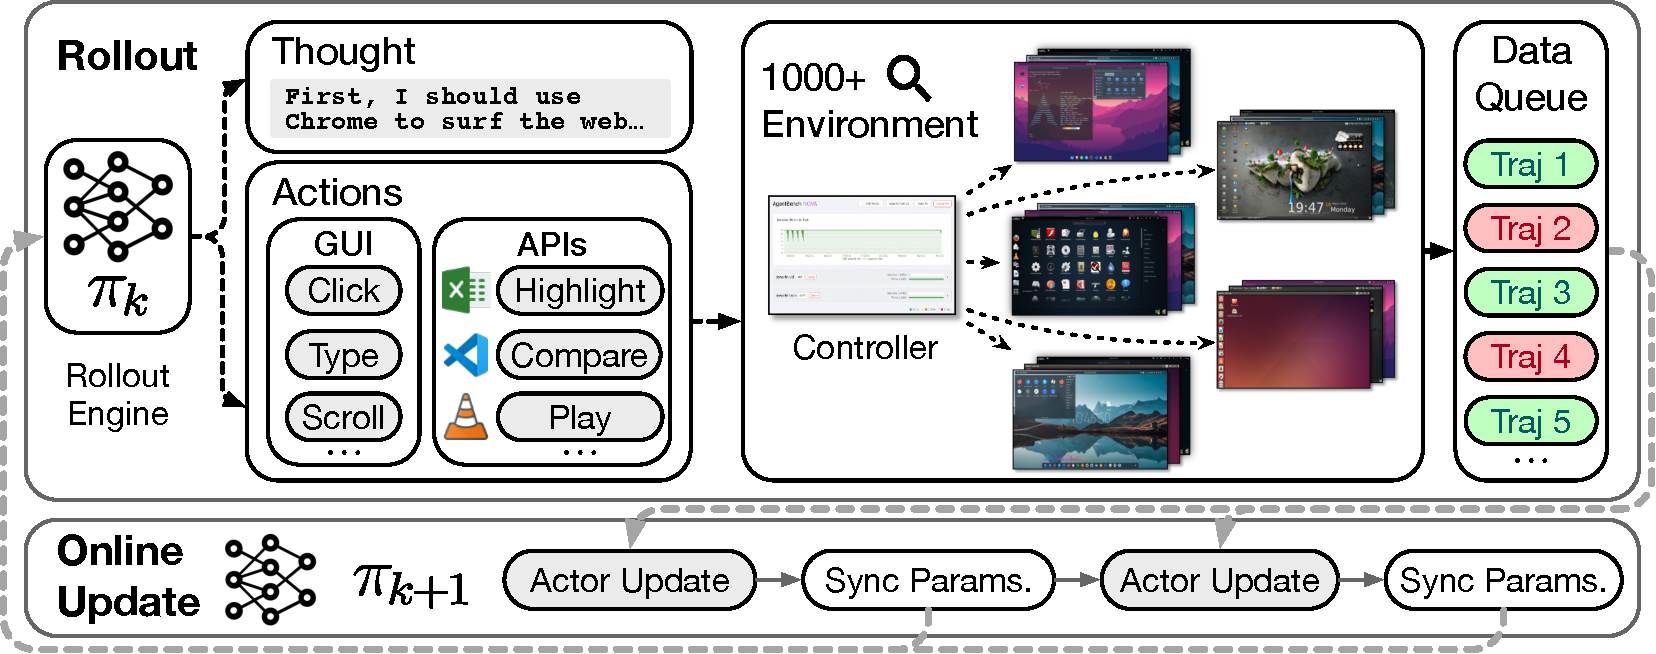
\includegraphics[width=0.95\textwidth]{images/framework.pdf}
    \caption{Overview of \computerrl framework. We introduce an API-GUI action paradigm that seamlessly integrates automatically constructed APIs with GUI actions to improve agent efficiency and effectiveness. A large-scale parallel desktop environment with 1,000+ real-world instances, combined with an asynchronous RL framework, enables efficient sampling and robust agent training.}
    \label{figs:framework}
    \vspace{-3mm}
\end{figure}

\subsection{General API-GUI Paradigm}\label{sec:hybrid-action-space}
Existing GUI agents face challenges due to their reliance on human-like interactions, while API-based control offers efficiency but introduces implementation complexity and security restrictions. To address these issues, we propose an API-GUI paradigm that unifies both action spaces, enabling agents to leverage API efficiency while retaining GUI versatility.

We develop an LLM-based automated workflow for application API development~\citep{yang2024swe,wang2024openhands}, significantly lowering the barrier for API creation. Users provide exemplar tasks, and our system autonomously generates API code and test cases through three stages:
\begin{itemize}[leftmargin=1.5em,itemsep=0pt,parsep=0.2em,topsep=0.0em,partopsep=0.0em]
    \item \textbf{Requirement Analysis}: Users provide task examples for the target application. Our LLM analyzes these instances, extracts essential functionalities, and compares against existing API interfaces to identify gaps. New interfaces are automatically generated for uncovered functionalities, with a focus on general-purpose functions to minimize complexity and enhance usability.

    \item \textbf{API Implementation}: The workflow iterates over each interface definition, implementing API functionalities using designated Python libraries. Error-handling mechanisms and logging are implemented for debugging and maintenance purposes.

    \item \textbf{Test Case Generation}: Similar to \citet{li2024largelanguagemodelstest}, we verify API correctness by checking: (1) runtime error-free invocation and (2) correct results across parameter inputs; failed APIs receive error feedback for autonomous correction.
\end{itemize}

This methodology enables the creation of application-specific APIs with minimal human intervention. We have developed API sets for multiple Ubuntu applications and validated their effectiveness through experiments. Detailed API development workflow is provided in Appendix~\ref{apdx:api_construction}.
The agent action space and prompt formulation are detailed in Appendix~\ref{apdx:action_space} and~\ref{apdx:agent_prompt}.
    
\subsection{Stable Ubuntu Environment for Large-Scale Parallelism}\label{sec:stable-ubuntu}
A stable and scalable Ubuntu environment is essential for constructing behavior cloning data and large-scale RL training. Building on OSWorld~\citep{xie2024osworld}, we identify key limitations:

\begin{itemize}[leftmargin=1.5em,itemsep=0pt,parsep=0.2em,topsep=0.0em,partopsep=0.0em]
    \item \textbf{Resource Intensiveness and Stability}: VMs are CPU-intensive and unstable under high concurrency, causing performance degradation and system freezes.
    \item \textbf{Network Bottlenecks}: Heavy workloads cause network overhead, connection failures, and IP address loss, hindering agent interaction and logging.
    \item \textbf{Lack of Native Distributed Support}: OSWorld lacks multi-node clustering support, preventing efficient distributed deployment.
\end{itemize}

To address these limitations, we build a robust and parallelizable OSWorld infrastructure (see Figure~\ref{figs:framework}) with the following innovations:
\begin{itemize}[leftmargin=1.5em,itemsep=0pt,parsep=0.2em,topsep=0.0em,partopsep=0.0em]
    \item \textbf{Standardized, Decoupled Interface}: We refactor the environment via AgentBench API, providing a unified interface that decouples environment execution from the computational back-end and enables flexible resource management.
    \item \textbf{Lightweight VM Deployment}: Using \href{https://github.com/qemus/qemu}{\texttt{qemu-in-dockere}}, we deploy containerized Ubuntu VMs with streamlined images that reduce network issues and optimize resource usage, significantly lowering per-instance CPU consumption.
    \item \textbf{Distributed Multi-Node Clustering}: We employ \href{https://github.com/grpc}{gRPC-based} communication to link CPU nodes into a distributed cluster with centralized resource allocation and orchestration.
    \item \textbf{Web-based Visualization and Monitoring}: A web interface provides real-time visualization of environment statuses, agent states, and resource allocation, improving usability and debugging capabilities.
\end{itemize}

Through these technical improvements, our system supports deployment of \textbf{several thousands} of concurrent environments on a multi-node CPU cluster, as validated by extensive empirical evaluation. Results confirm our platform’s superior stability, resource efficiency, and scalability, making it an enabling infrastructure for large-scale RL and agent-based research.

\subsection{Full-Asynchronous RL Framework for Efficient Training}\label{sec:full-asynchronous}
Existing RL frameworks rely on synchronous training paradigms, where rollout collection and parameter updates are alternated, resulting in training inefficiencies. To address the limitation, we use the AgentRL framework~\citep{zhang2025model} for fully asynchronous RL training with the following designs:

\begin{itemize}[leftmargin=1.5em,itemsep=0pt,parsep=0.2em,topsep=0.0em,partopsep=0.0em]
    \item \textbf{Resource Partitioning}: Data collection runs on dedicated resources while the trainer streams data from the replay engine, preventing mutual blocking.
    \item \textbf{Dynamic Batch Sizing}: The trainer processes incoming data with flexible batch sizes, reducing idle time and improving efficiency.
    \item \textbf{Modular Component Isolation}: Actor, reference, and critic modules run independently with dedicated resources. We utilize PyTorch distributed groups and NCCL for efficient parameter sharing.
    \item \textbf{Off-policy Bias Mitigation}: We limit the replay buffer size and sync trajectories after each update, ensuring trajectories remain close to the latest policy.
\end{itemize}

Through a stable, high-concurrency desktop environment and the decoupling of training from rollout, we markedly enhance the efficiency of sampling and RL training. Our system achieves a high average power consumption per GPU, reflecting optimal resource utilization. This design supports scalable, high-throughput RL training by enabling dynamic workload balancing, resulting in a significant improvement in hardware efficiency and overall training throughput.